\section*{\textbf{April 2 (Sarah)}}
Goals of the course:
\begin{enumerate}[(i)]
\item We would like to develop basic Hamiltonian Floer theory in such a way that we understand what we are blackboxing and where in the literature we would find the proofs. We would also like to keep Morse theory running in parallel for comparison's sake.

\item We would like to discuss some recent developments in the theory.
\end{enumerate}

Fundamental analytic program for obtaining moduli spaces which lead to invariants in Floer or Morse theory (see Schwarz's book):
\begin{enumerate}[(1)]
\item analytic setup, definition of functional spaces of solutions/trajectories (moduli spaces are cut out by equations)

\item analyze the index problem (ideally, we want to think of our spaces as finite-dimensional manifolds, and the index should theoretically give the dimension)

\item transversality (we want to give our spaces ``manifold-like'' structures)

\item compactness (we want to be able to count things, and counts need to be finite)

\item gluing (if we add points to compactify, they should have neighborhoods which look appropriately manifold-like; this is a sort of converse to compactness)

\item coherent orientations (when we count, we want to keep track of sign)
\end{enumerate}

\bigskip

Today we start with an exercise in Morse theory; it will illustrate steps (1), (2), and (3).

\begin{thm}[Local stable manifold theorem]
Let $\varphi:\R^n\arr\R$ be a smooth function whose only critical point is $0$. We assume that this critical point is Morse, in the sense that the Hessian at this point is non-degenerate. Fix a Riemannian metric $g$ on $\R^n$, and let $\gr$ be the gradient of $\phi$ with respect to $g$. Let $S \subset \R^n$ be the stable set of $0$ (that is, the set of points which flow to $0$ under $-\gr$). Then $S$ is a submanifold of $\R^n$ near $0$.
\end{thm}

\begin{remark}
Other proofs of this theorem are also hard. For instance, look up the Hartman-Grobman theorem and note how this does not follow from it.
\end{remark}

\newpage

\begin{example}
Consider the function $\phi:\R^2\arr\R$ given by $\phi(x,y)=x^2-y^2$. Then $\phi$ is Morse, and its only critical point is $(0,0)$. Here's a drawing of the flow lines:
\begin{center}
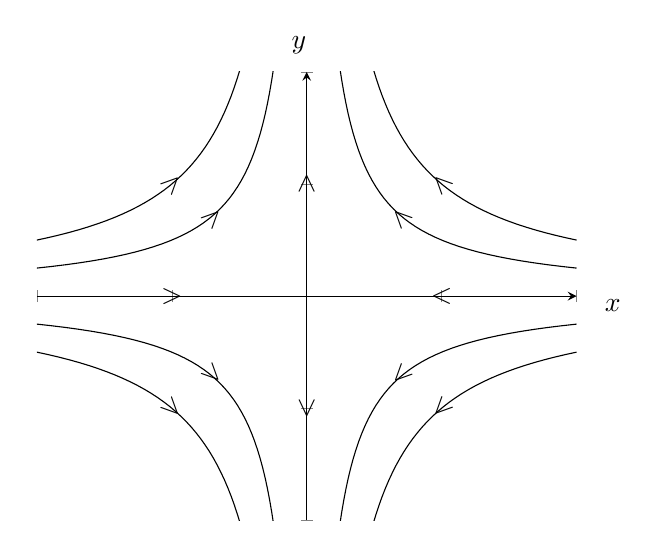
\begin{tikzpicture}

\begin{axis}[ymin=-1,ymax=1,xmax=1,xmin=-1,xticklabel=\empty,yticklabel=\empty,axis lines = middle,xlabel=$x$,ylabel=$y$,label style ={at={(ticklabel cs:1.1)}}]

\addplot[samples=50, no markers, domain=0:1.04] ({exp(-2*x))},{0.25*exp(2*x))});
\addplot[samples=50, no markers, domain=0:1.39] ({exp(-2*x))},{0.125*exp(2*x))});

\addplot[samples=50, no markers, domain=0:1.04] ({-exp(-2*x))},{0.25*exp(2*x))});
\addplot[samples=50, no markers, domain=0:1.39] ({-exp(-2*x))},{0.125*exp(2*x))});

\addplot[samples=50, no markers, domain=0:1.04] ({-exp(-2*x))},{-0.25*exp(2*x))});
\addplot[samples=50, no markers, domain=0:1.39] ({-exp(-2*x))},{-0.125*exp(2*x))});

\addplot[samples=50, no markers, domain=0:1.04] ({exp(-2*x))},{-0.25*exp(2*x))});
\addplot[samples=50, no markers, domain=0:1.39] ({exp(-2*x))},{-0.125*exp(2*x))});

\node [rotate=0] at (-0.5,0) {$>$};
\node [rotate=180] at (0.5,0) {$>$};
\node [rotate=90] at (0,0.5) {$>$};
\node [rotate=270] at (0,-0.5) {$>$};
\node [rotate=135] at (0.35,0.35) {$>$};
\node [rotate=135] at (0.5,0.5) {$>$};
\node [rotate=45] at (-0.35,0.35) {$>$};
\node [rotate=45] at (-0.5,0.5) {$>$};
\node [rotate=-45] at (-0.35,-0.35) {$>$};
\node [rotate=-45] at (-0.5,-0.5) {$>$};
\node [rotate=-135] at (0.35,-0.35) {$>$};
\node [rotate=-135] at (0.5,-0.5) {$>$};

\end{axis}

\end{tikzpicture}
\end{center}
Thus the stable set is the $x$-axis.
\end{example}

Now we proceed to the proof of the stable manifold theorem.

For $x \in \R^n$, the gradient flow line starting at $x$ is the (unique) path $\gamma_x:[0,\delta) \arr \R^n$ such that $\gamma(0)=x$, $\dot{\gamma}(t)=-\gr(\gamma(t))$, and $\delta>0$ is maximal. Note that for $x \in S$, $\delta=\oo$.

The plan is to do the following:
\begin{itemize}
\item Identify $S \subset \R^n$ with the set of smooth gradient flow lines starting at points in $S$.

\item Construct a path space $P$ (a Banach manifold) and a Banach space bundle $\mathscr{E} \arr P$.

\item Define a (Fredholm) section $s:P \arr \mathscr{E}$, $\gamma \mapsto \dot{\gamma}+\gr \circ \gamma$ such that $s^{-1}(0)=S$ (this will be non-trivial because $P$ is large).

\item Prove $s \pitchfork 0$ and use the implicit function theorem. This will use a baby version of the Atiyah-Patodi-Singer index theorem.
\end{itemize}
First, we define our Banach space to be the Sobolev space $P=W^{1,2}(\R_{\geq 0},\R^n)$. Observe that $P$ can also be written as the equivalence classes of functions $f:\R_{\geq 0}\arr\R^n$ which are square-integrable and have weak derivatives $f'$ which are also square-integrable. In this special case, we mean that $f$ is differentiable almost everywhere, and 
\[
f(t) = f(0) + \displaystyle\int_0^t f'(s) \, ds
\]
almost everywhere. 

Note that in higher dimensions, we'll have to be more mature about how we define these spaces.

\newpage

\begin{prop} \label{cptim}
  If $\gamma \in W^{1,2}(\R_{\geq 0},\R^n)$, then $\gamma(t) \arr 0$ as $t \arr \oo$.
\end{prop}
\begin{proof}
The basic idea is that the finiteness of the $(1,2)$-norm gives certain bounds on the first derivative, which forces the variance to approach zero. Then the $(1,2)$-norm also forces the values of the function itself to go to zero.

The hypothesis $\gamma \in W^{1,2}(\R_{\geq 0},\R^n)$ tells us that the values
\[
\left( \displaystyle\int_0^\oo |\gamma|^2 \right)^{1/2} = \left( \sumto{N=0}{\oo} \displaystyle\int_N^{N+1} |\gamma|^2 \right)^{1/2}
\]
and
\[
\left( \displaystyle\int_0^\oo |\dot{\gamma}|^2 \right)^{1/2} = \left( \sumto{N=0}{\oo} \displaystyle\int_N^{N+1} |\dot{\gamma}|^2 \right)^{1/2}
\]
are finite. It follows that 
\[
\displaystyle\int_N^{N+1} |\gamma|^2 \qquad \text{and} \qquad \displaystyle\int_N^{N+1} |\dot{\gamma}|^2 \tag{$\dagger$} \label{01ints}
\]
approach zero as $N \arr \oo$.

Since $\dot{\gamma}$ is a weak derivative, for almost every $x \in [N,N+1]$ we have
\begin{align*}
|\gamma(x)-\gamma(N)| & = \left| \displaystyle\int_N^x \dot{\gamma} \right|
\\
& \leq \rt{x-N} \left( \displaystyle\int_N^x |\dot{\gamma}|^2 \right)^{1/2}
\\
& \leq \rt{x-N} \left( \displaystyle\int_N^{N+1} |\dot{\gamma}|^2 \right)^{1/2}
\\
& \leq \left( \displaystyle\int_N^{N+1} |\dot{\gamma}|^2 \right)^{1/2}
\end{align*}
(the second line follows from Cauchy-Schwarz). Combining this information with the fact that both expressions in (\ref{01ints}) go to zero yields the desired result.
\end{proof}
\begin{remark}
We have constructed a version of the Rellich embedding $W^{1,2}(\R,\cdot) \hookrightarrow C^0(\R,\cdot)$, which sends Sobolev spaces to H\"{o}lder spaces.
\end{remark}

\begin{remark}
In the general case, we'll need to build asymptotic conditions by hand. This makes it difficult to turn more general analogues of $P$ into Banach manifolds.
\end{remark}

Now let $\mathscr{E}=P \times L^2(\R_{\geq 0},\R^n)$, so $\mathscr{E} \arr P$ is a trivial bundle. Define a section $s:P \arr \mathscr{E}$ by $s(\gamma)=(\gamma, \dot{\gamma}+\gr \circ \gamma)$. We do need to check that $\gr \circ \gamma$ is square-integrable, but this shouldn't be too bad because $\gr$ is smooth and $\gamma$ has compact image by Proposition~\ref{cptim}. We will also need to demonstrate some kind of regularity for $s$.

\begin{prop} \label{zeroSet}
If $\gamma \in S$ (i.e., $\gamma$ is a smooth gradient flow line starting at a point in $S$), then $\gamma \in P=W^{1,2}(\R_{\geq 0},\R^n)$. Moreover, $S=s^{-1}(0)$.
\end{prop}

In order to prove Proposition~\ref{zeroSet}, we will need the following lemma (which we will blackbox for now).

\begin{lemma}[Exponential convergence of flow lines at the ends] \label{expConv}
If $\gamma \in S$, then there is some $a>0$ so that $|\gamma(t)| \leq e^{-at}$.
\end{lemma}

\begin{remark}
Using the gradient flow line equation we obtain the same exponential convergence result for all derivatives of flow lines. This uses a method called \emph{bootstrapping}.
\end{remark}

If $\gamma \in S$, then Lemma~\ref{expConv} tells us $\gamma \in P$, so we have $S \subset s^{-1}(0)$. On the other hand, we still need to check that if $f \in P$ satisfies $s(f)=0$, then $f$ is a smooth gradient flow line starting at a point in $S$. The tricky part is verifying that $f$ is smooth. The Rellich embedding $W^{1,2}(\R_{\geq 0},\R^n) \hookrightarrow C^0(\R_{\geq 0},\R^n)$ forces $f$ to be continuous. Then we use bootstrapping to guarantee that $f$ is actually smooth. We know that $f$ has a weak derivative. Since $f$ is a continuous solution of the gradient flow line equation, we can show that $f$ has a genuine derivative $f$' which must also be continuous. Repeating this process infinitely shows that $f$ is, in fact, smooth.
